\documentclass{beamer}

\usepackage{array}
\usepackage{amsmath}
\usepackage{amssymb}
\usepackage{mathtools}
\usepackage{textcomp}
\usepackage{gensymb}
\usepackage{graphicx}
\usepackage{float}
\usepackage{caption}
\usepackage{amsfonts}
\usepackage[margin=1in]{geometry}
% \newcommand\df[1]{\index{#1@\myupper #1}{{\bf{#1}}}}
% \newcommand\myupper[1]{\uppercase{#1}}

% \newcommand\myscalar[1]{#1}
\newcommand\myvector[1]{\mathbf{#1}}
\newcommand\mymatrix[1]{\mathbf{#1}}

% \newcommand\mytensor[1]{{\textit{\textsf{\uppercase{#1}}}}}

% \newcommand\myrvscalar[1]{\textrm{#1}}
% \newcommand\myrvvector[1]{\textbf{#1}}
% \newcommand\myrvmatrix[1]{{\textbf{\uppercase{#1}}}}
% \newcommand\myrvtensor[1]{{{\textsf{\uppercase{#1}}}}}

% \newcommand\gup[1]{\textrm{\greektext p}}




\newcommand{\df}[2][]{%
  \ifthenelse{\isempty{#1}}%
    {\index{#2@\myupper #2}{{\bf{#2}}}}% if #1 is empty
    {\index{#2@\myupper #1}{{\bf{#2}}}}% if #1 is not empty
}
\newcommand\myupper[1]{\uppercase{#1}}



\newcommand\twobytwo[4]{\left[\begin{array}{cc}
#1 & #2 \\
#3 & #4 
\end{array}\right]}

\newcommand{\intR}{\int_{-\infty}^{\infty}}
\newcommand{\bounds}[2]{\biggr\rvert_{#1}^{#2}}
\newcommand{\eval}[1]{\biggr\rvert_{#1}}
\newcommand{\opp}[1]{\mathrm{\bf{#1}}}

\newcommand{\Lim}[1]{\raisebox{0.5ex}{\scalebox{0.8}{$\displaystyle \lim_{#1}\;$}}}

\let\origref=\ref

\renewcommand{\ref}[1]{(\origref{#1})}
\newcounter{results}
\newcounter{questions}

\def\neg{{\sim}}
\def\Z{\mathbb{Z}}
\def\N{\mathbb{N}}
\def\R{\mathbb{R}}
\def\Q{\mathbb{Q}}
\def\E{\mathbb{E}}
\def\qed{\(\blacksquare\)}
\newcommand{\result}[1]{\stepcounter{results}{\bfseries Result \arabic{results}}: #1}
\newcommand{\question}[1]{\stepcounter{questions}{\bf \arabic{questions}}: #1}


\def\limfunc{\frac{x^2-1}{x-1}}

\def\oneoverx{\frac{1}{x}}

%Information to be included in the title page:
\title{The Method of Green's Functions}
\author{Ryan Coyne}
\institute[NHTI]{NHTI-Concord's Community College}
\date{5/5/2023}

\begin{document}

\frame{\titlepage}

\section*{Calculus}

    \begin{frame}
    \frametitle{The Limit}
        \(f(x)=\limfunc\)\\[28.5pt]
        \begin{figure}
            \centering
            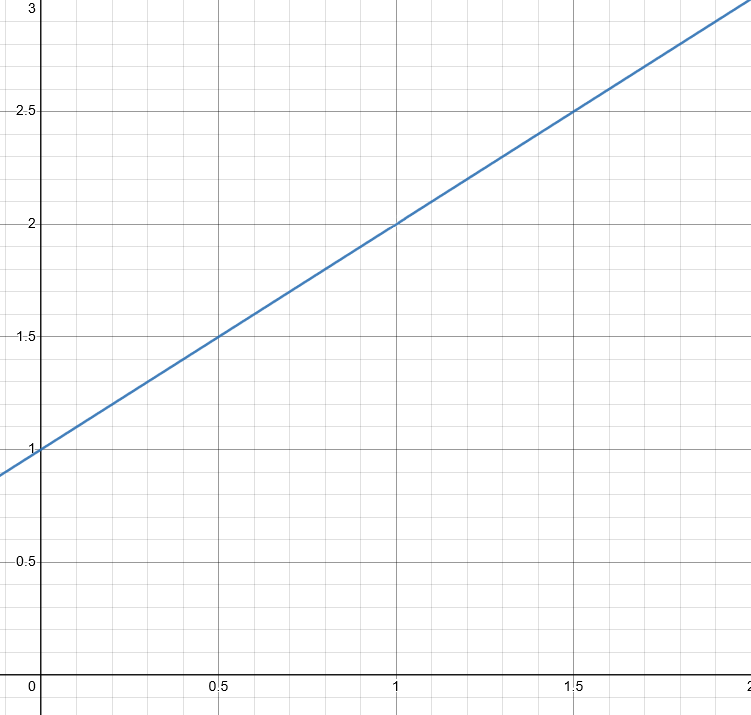
\includegraphics[width=0.6\linewidth]{include/images/limit_1.png}
        \end{figure}
    \end{frame}

    \begin{frame}
        \frametitle{The Limit}
        \(f(x)=\limfunc\)\\
        \(f(1)=\frac{1^2-1}{1-1}=\frac{0}{0}\)\\[12pt]
        \begin{figure}
            \centering
            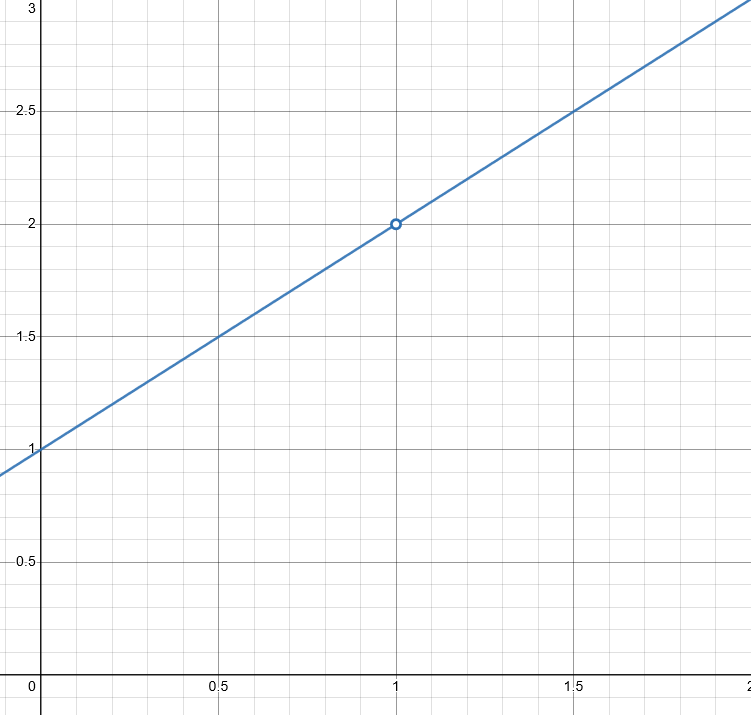
\includegraphics[width=0.6\linewidth]{include/images/limit_2.png}
        \end{figure}
    \end{frame}

    \begin{frame}
        \frametitle{The Limit}
        \(f(x)=\limfunc\)\\
        \(f(1)=\frac{1^2-1}{1-1}=\frac{0}{0}\)\\[12pt]
        \begin{figure}
            \centering
            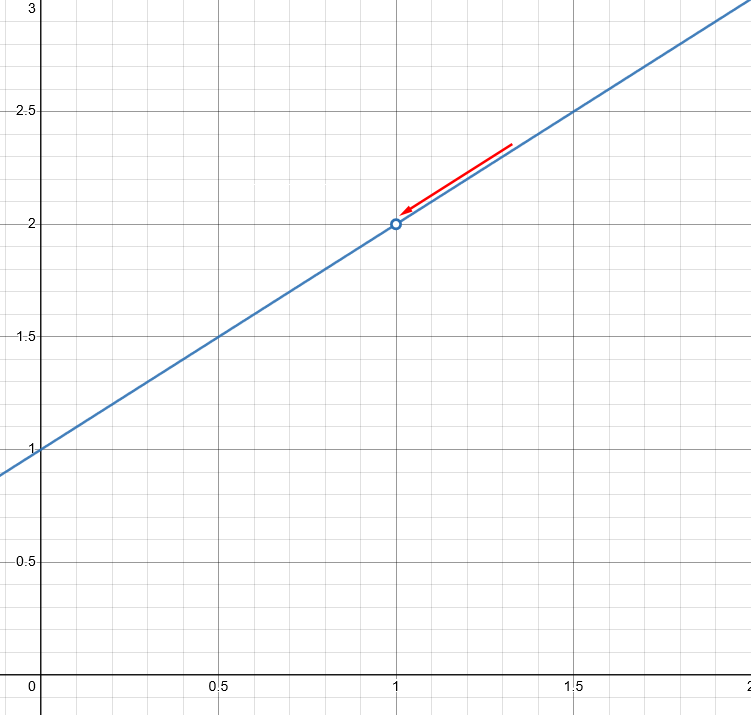
\includegraphics[width=0.6\linewidth]{include/images/limit_3.png}
        \end{figure}
    \end{frame}

    \begin{frame}
        \frametitle{The Limit}
        \(f(x)=\limfunc\)\\
        \(f(1)=\frac{1^2-1}{1-1}=\frac{0}{0}\)\\[12pt]
        \begin{figure}
            \centering
            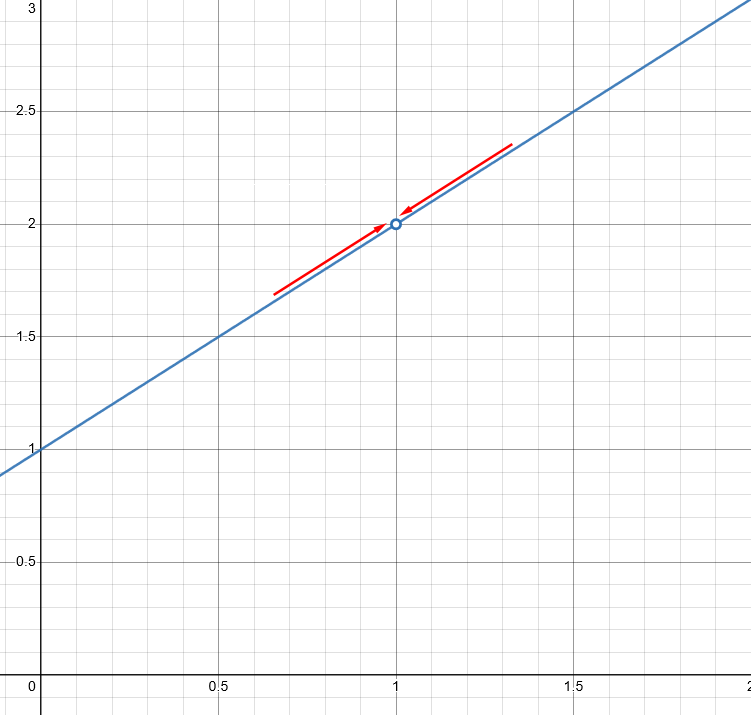
\includegraphics[width=0.6\linewidth]{include/images/limit_4.png}
        \end{figure}
    \end{frame}

    \begin{frame}
        \frametitle{The Limit}
        \(\Lim{x\to 1}\limfunc = 2\)\\[28.5pt]
        \begin{figure}
            \centering
            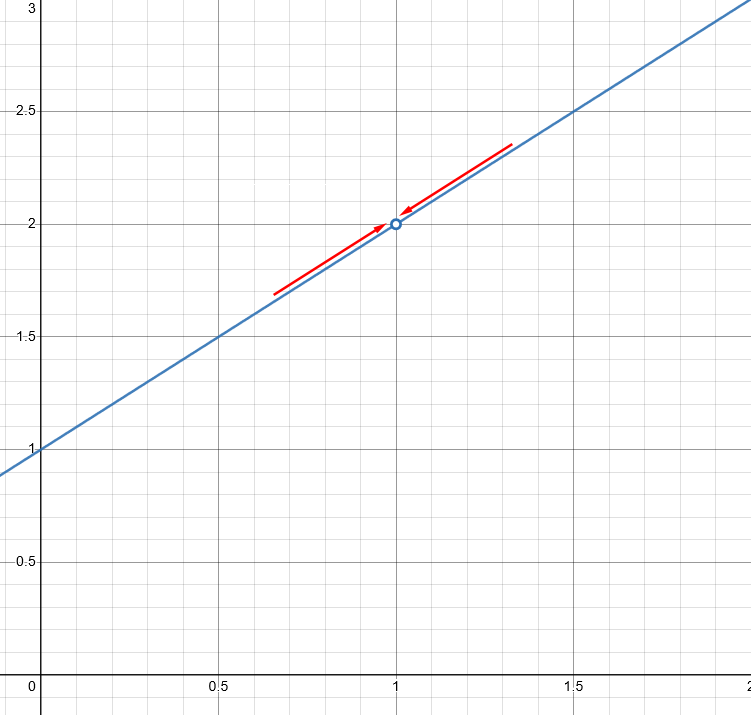
\includegraphics[width=0.6\linewidth]{include/images/limit_4.png}
        \end{figure}
    \end{frame}

    \begin{frame}
        \frametitle{The Limit}
        \(f(x)=\oneoverx\)\\
        \begin{figure}
            \centering
            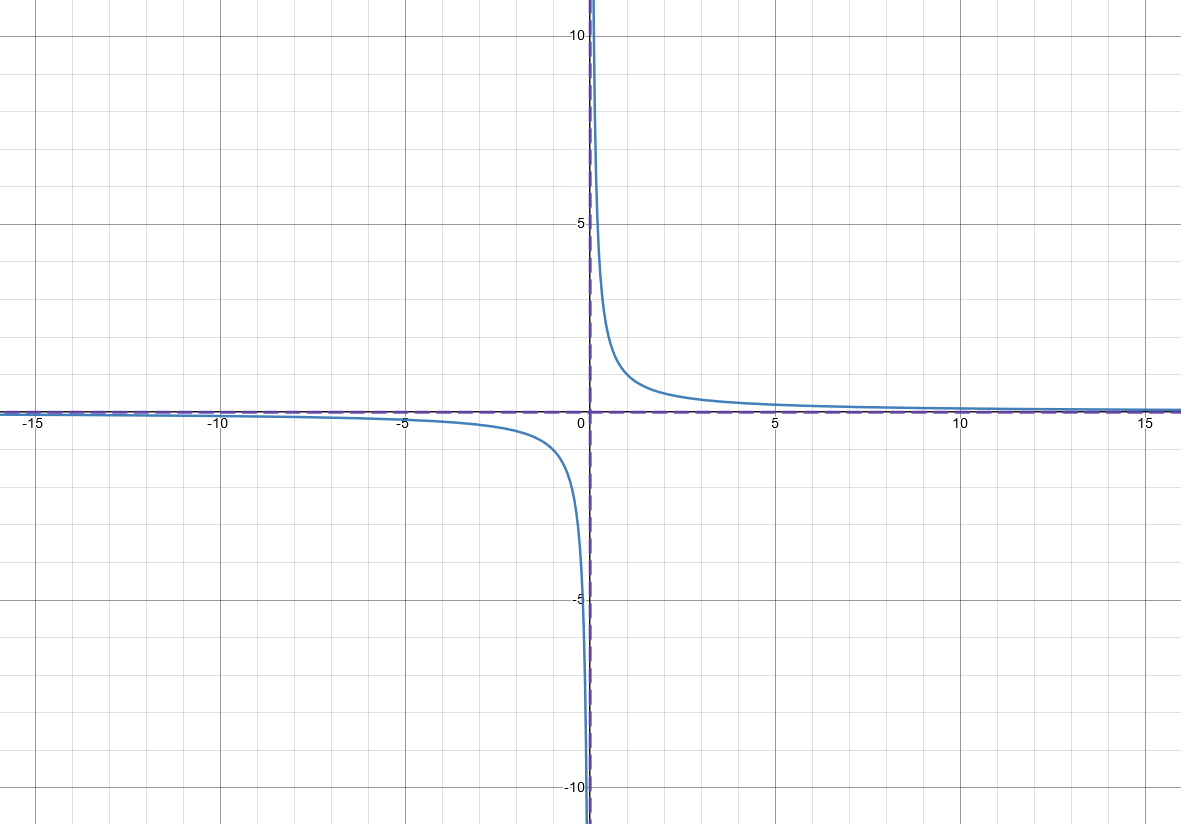
\includegraphics[width=0.75\linewidth]{include/images/invx_1.png}
        \end{figure}
    \end{frame}

    \begin{frame}
        \frametitle{The Derivative}
        \(f(x)=x+1\)\\[28.5pt]
        \begin{figure}
            \centering
            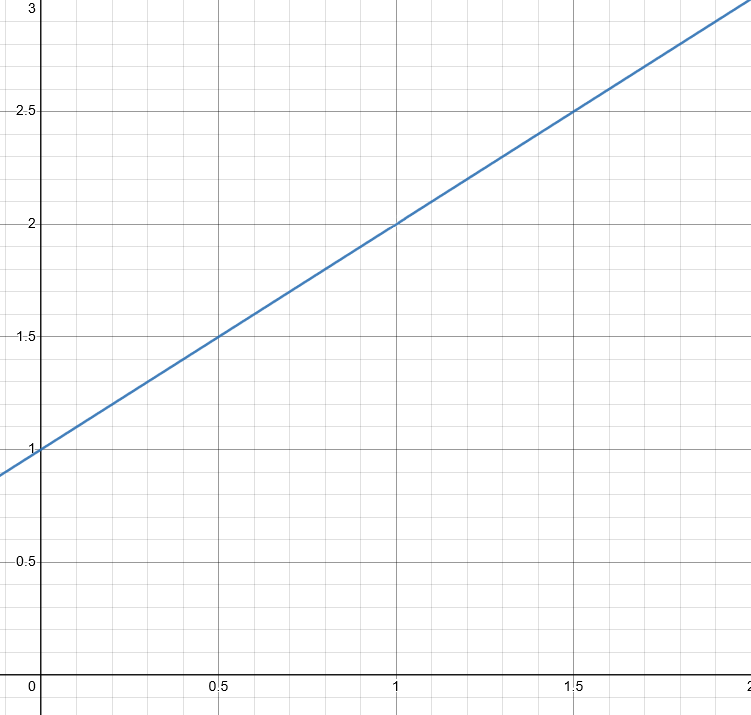
\includegraphics[width=0.6\linewidth]{include/images/limit_1.png}
        \end{figure}
    \end{frame}

    \begin{frame}
        \frametitle{The Derivative}
        \(f(x)=\frac{1}{x}\)\\[26pt]
        \begin{figure}
            \centering
            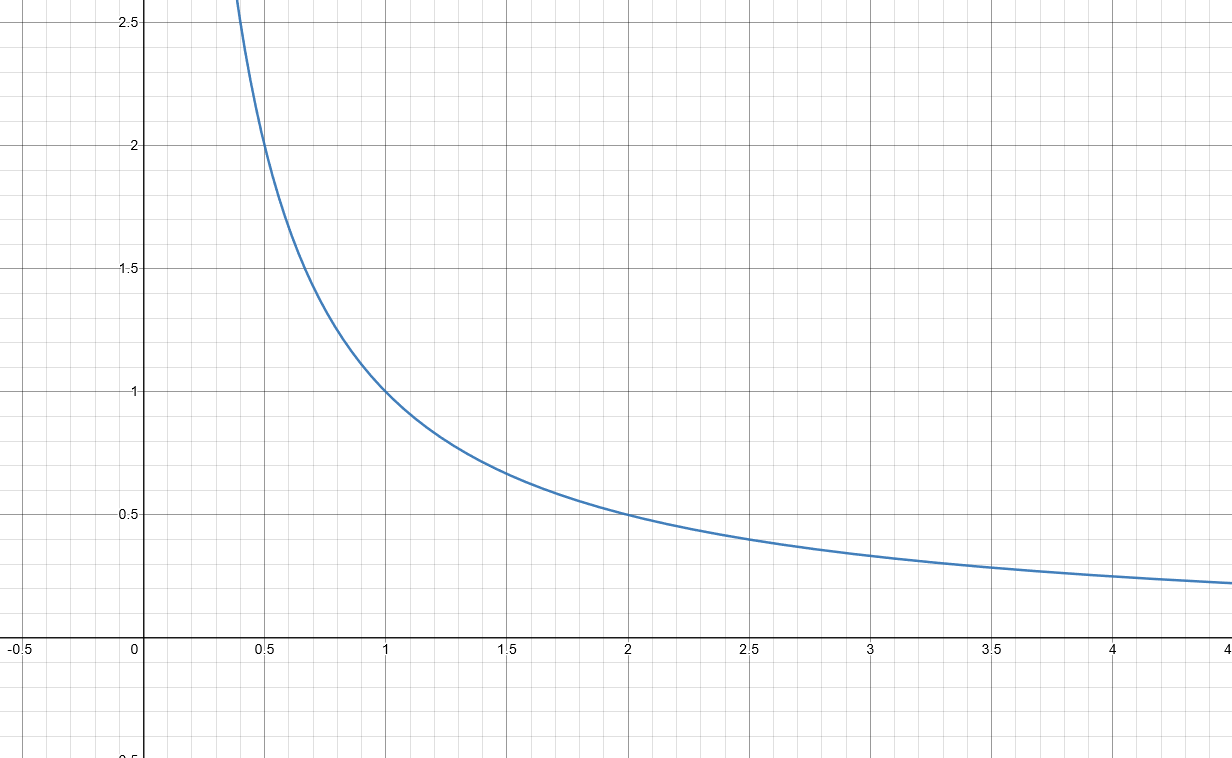
\includegraphics[width=0.6\linewidth]{include/images/invx_2.png}
        \end{figure}
    \end{frame}

    \begin{frame}
        \frametitle{The Derivative}
        \(f(x)=\frac{1}{x}\)\\
        \(f'(x)=-\frac{1}{x^2}\)\\[12pt]
        \begin{figure}
            \centering
            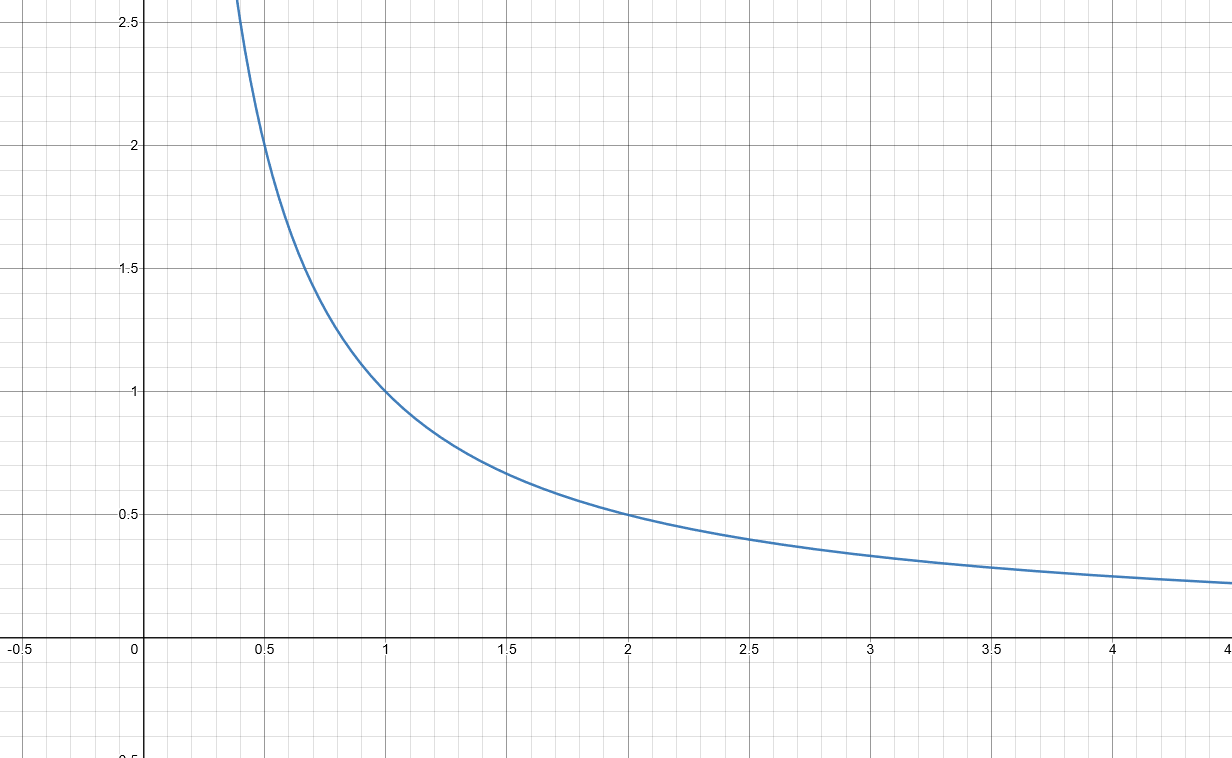
\includegraphics[width=0.6\linewidth]{include/images/invx_2.png}
        \end{figure}
    \end{frame}

    \begin{frame}
        \frametitle{The Derivative}
        \(f(x)=\frac{1}{x}\)\\
        \(f'(x)=-\frac{1}{x^2}\)\\
        \(f'(1)=1\)\\
        \begin{figure}
            \centering
            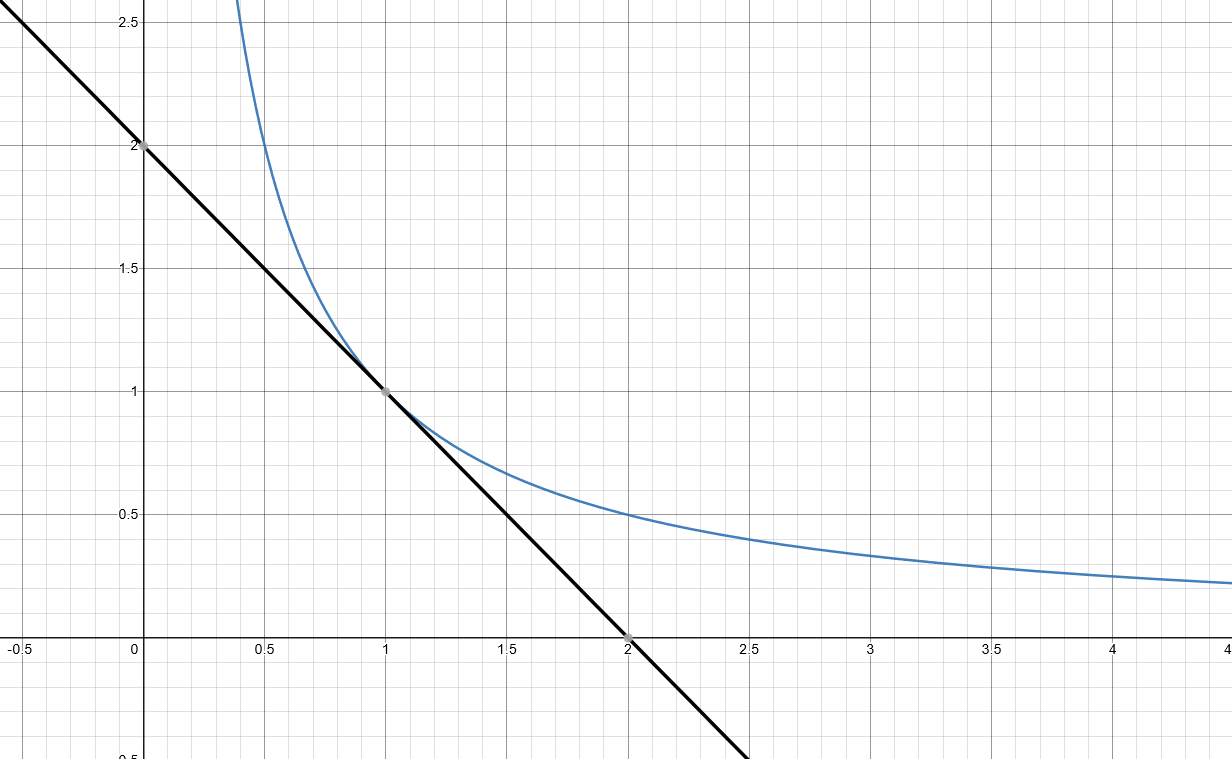
\includegraphics[width=0.6\linewidth]{include/images/invx_3.png}
        \end{figure}
    \end{frame}

    \begin{frame}
        \frametitle{The Anti-Derivative}
        \(\int f(x)dx = F(x)\)\\[12pt] \pause
        \(f(x)=\frac{1}{x}\)\\[12pt]
        \(\int \frac{1}{x} dx = \ln x +c\)
    \end{frame}

    \begin{frame}
        \frametitle{The Integral}
        \(f(x)=\frac{1}{x}\)\\[26pt]
        \begin{figure}
            \centering
            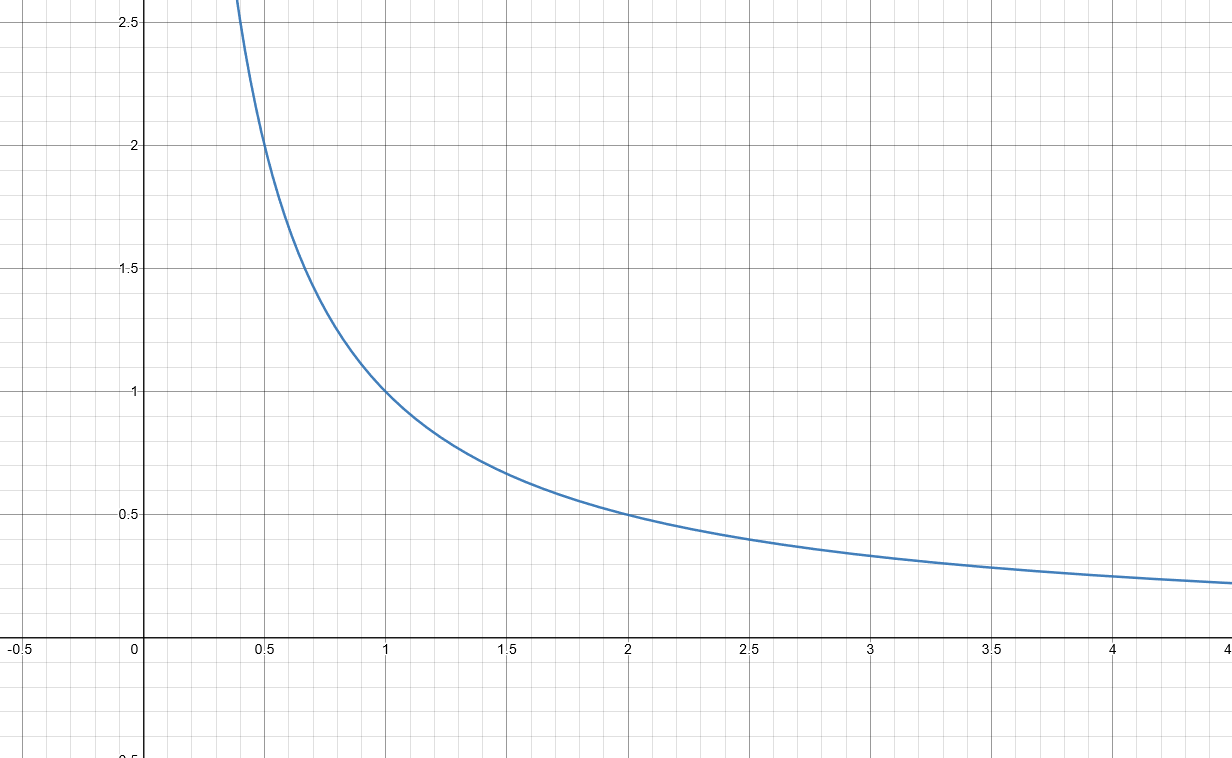
\includegraphics[width=0.6\linewidth]{include/images/invx_2.png}
        \end{figure}
    \end{frame}

    \begin{frame}
        \frametitle{The Integral}
        \(f(x)=\frac{1}{x}\)\\[26pt]
        \begin{figure}
            \centering
            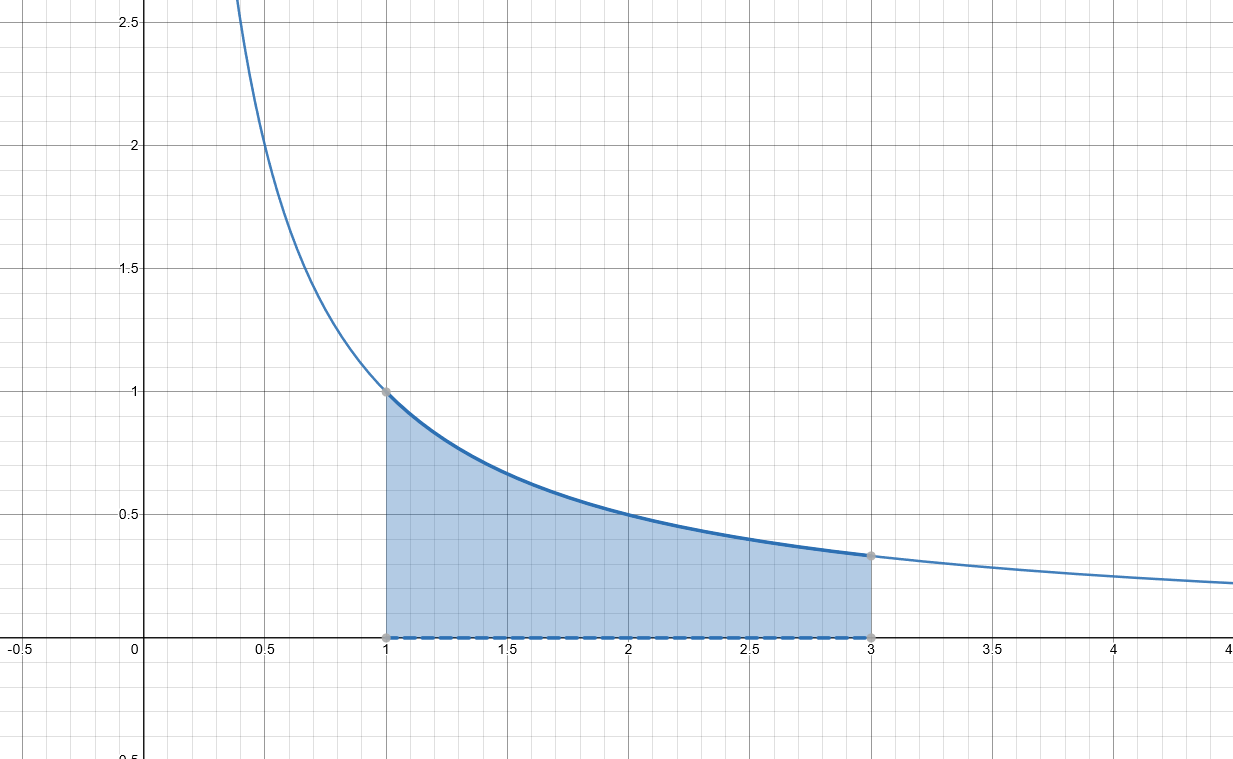
\includegraphics[width=0.6\linewidth]{include/images/invx_4.png}
        \end{figure}
    \end{frame}

    \begin{frame}
        \frametitle{The Integral}
        \(\int_\lima^\limb f(x) dx = F(a) - F(b)\)\\
    \end{frame}

    \begin{frame}
        \frametitle{The Integral}
        \(f(x)=\frac{1}{x}\)\\
        \(\int_1^3 f(x) dx = F(3) - F(1)\)\\
        \(\hspace{49pt}=\ln(3)-\ln(1)\)
        \begin{figure}
            \centering
            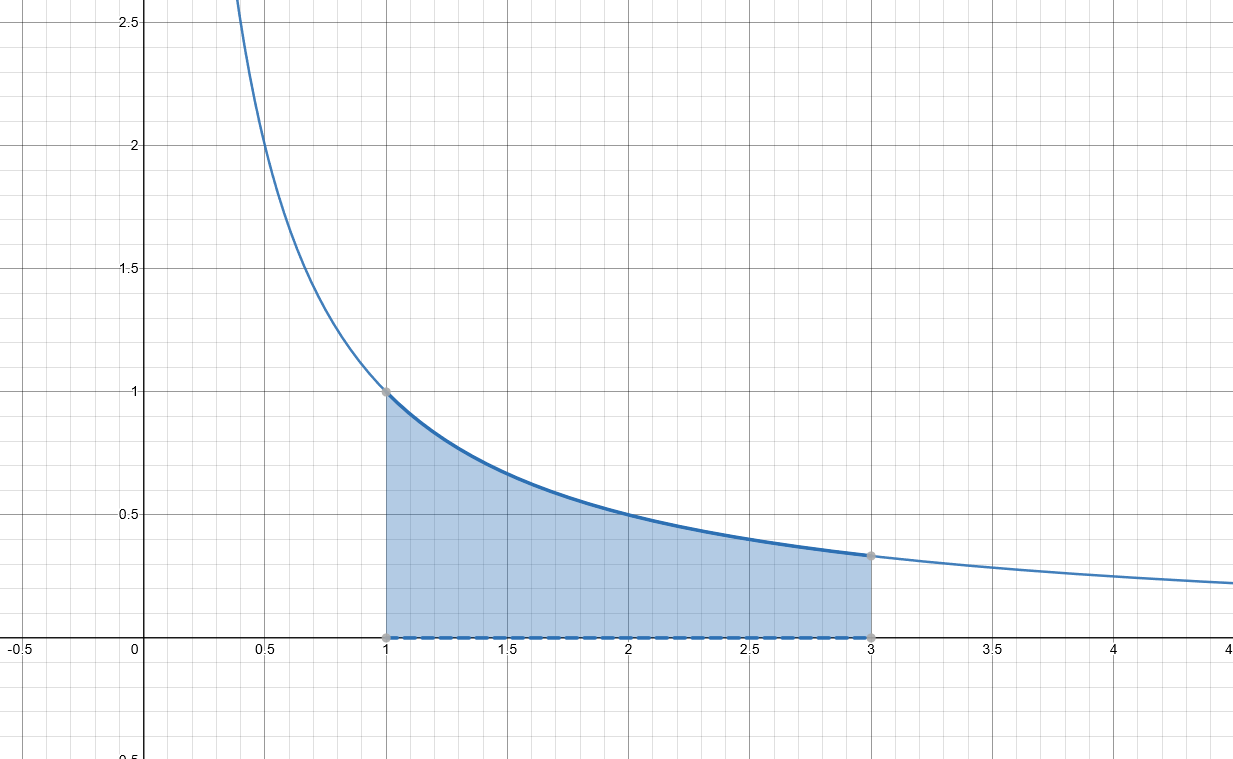
\includegraphics[width=0.6\linewidth]{include/images/invx_4.png}
        \end{figure}
    \end{frame}

    \begin{frame}
        \frametitle{Differential Equations}
        
        
    
    \end{frame}

    \begin{frame}
        \frametitle{The Adjoint Operator}
    
        
    
    \end{frame}

    \begin{frame}
        \frametitle{The Dirac Delta Function}
    
        
    
    \end{frame}
    
    \begin{frame}
        \frametitle{The Method of Green's Functions}
    
        
    
    \end{frame}
    
\end{document}